\documentclass[tikz,border=10pt]{standalone}
\usetikzlibrary{calc}
\begin{document}
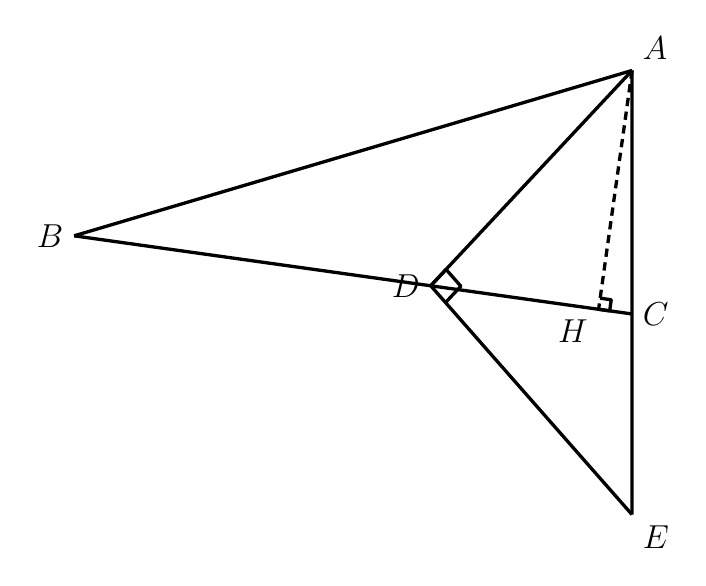
\begin{tikzpicture}[line width=1.2pt, line join=round]
% Coordinates in cm: x=(px-300)*0.014981, y=(254-py)*0.014981 (y flipped)
\coordinate (A) at (3.6122739231153185,2.818336258210227);
\coordinate (B) at (-3.473072483431232,0.7184354646595663);
\coordinate (C) at (3.6115734119036267,-0.2740176435128856);
\coordinate (D) at (1.0558236222666029,0.0840047417846746);
\coordinate (H) at (3.1874051188188766,-0.21459799896334442);
\coordinate (E) at (3.610996407326808,-2.821160822178238);

% Right-angle square at H (mark points converted from pixels)
\coordinate (P1) at (3.32799277538802,-0.23478443347948);
\coordinate (P2) at (3.34742250172661,-0.09379074620704);
\coordinate (P3) at (3.20670370945388,-0.07306946572160);

% Right-angle square at D for angle ADE (sides along DA and DE, 19 px)
\coordinate (Q1) at (1.249856850128865,0.29197410479776453);
\coordinate (Q2) at (1.4376344167312634,0.07877822040381142);
\coordinate (Q3) at (1.2436011888690013,-0.12919114260927855);

% Solid segments
\draw (A) -- (B);          % AB
\draw (B) -- (C);          % BC, passes through D
\draw (A) -- (E);          % vertical AC E
\draw (A) -- (D);          % AD
\draw (D) -- (E);          % DE

% Dashed altitude A-H
\draw[dash pattern=on 3pt off 2pt] (A) -- (H);

% Right-angle marks at H and D
\draw (H) -- (P1) -- (P2) -- (P3);
\draw (D) -- (Q1) -- (Q2) -- (Q3);

% Labels
\node[anchor=south west, font=\fontsize{12}{14.4}\selectfont] at (A) {$A$};
\node[anchor=east, font=\fontsize{12}{14.4}\selectfont] at (B) {$B$};
\node[anchor=west, font=\fontsize{12}{14.4}\selectfont] at (C) {$C$};
\node[left, font=\fontsize{12}{14.4}\selectfont] at (D) {$D$};
\node[anchor=north east, font=\fontsize{12}{14.4}\selectfont] at (H) {$H$};
\node[anchor=north west, font=\fontsize{12}{14.4}\selectfont] at (E) {$E$};
\end{tikzpicture}
\end{document}
% GEOAGENT_REPAIR_V1 c18a466396f54661 9bac344f1aea3e4dd02d2ae28bf22936b04aa47831382bbe8d392cc0a6f09df8